\documentclass{article}\usepackage[]{graphicx}\usepackage[]{xcolor}
% maxwidth is the original width if it is less than linewidth
% otherwise use linewidth (to make sure the graphics do not exceed the margin)
\makeatletter
\def\maxwidth{ %
  \ifdim\Gin@nat@width>\linewidth
    \linewidth
  \else
    \Gin@nat@width
  \fi
}
\makeatother

\definecolor{fgcolor}{rgb}{0.345, 0.345, 0.345}
\newcommand{\hlnum}[1]{\textcolor[rgb]{0.686,0.059,0.569}{#1}}%
\newcommand{\hlstr}[1]{\textcolor[rgb]{0.192,0.494,0.8}{#1}}%
\newcommand{\hlcom}[1]{\textcolor[rgb]{0.678,0.584,0.686}{\textit{#1}}}%
\newcommand{\hlopt}[1]{\textcolor[rgb]{0,0,0}{#1}}%
\newcommand{\hlstd}[1]{\textcolor[rgb]{0.345,0.345,0.345}{#1}}%
\newcommand{\hlkwa}[1]{\textcolor[rgb]{0.161,0.373,0.58}{\textbf{#1}}}%
\newcommand{\hlkwb}[1]{\textcolor[rgb]{0.69,0.353,0.396}{#1}}%
\newcommand{\hlkwc}[1]{\textcolor[rgb]{0.333,0.667,0.333}{#1}}%
\newcommand{\hlkwd}[1]{\textcolor[rgb]{0.737,0.353,0.396}{\textbf{#1}}}%
\let\hlipl\hlkwb

\usepackage{framed}
\makeatletter
\newenvironment{kframe}{%
 \def\at@end@of@kframe{}%
 \ifinner\ifhmode%
  \def\at@end@of@kframe{\end{minipage}}%
  \begin{minipage}{\columnwidth}%
 \fi\fi%
 \def\FrameCommand##1{\hskip\@totalleftmargin \hskip-\fboxsep
 \colorbox{shadecolor}{##1}\hskip-\fboxsep
     % There is no \\@totalrightmargin, so:
     \hskip-\linewidth \hskip-\@totalleftmargin \hskip\columnwidth}%
 \MakeFramed {\advance\hsize-\width
   \@totalleftmargin\z@ \linewidth\hsize
   \@setminipage}}%
 {\par\unskip\endMakeFramed%
 \at@end@of@kframe}
\makeatother

\definecolor{shadecolor}{rgb}{.97, .97, .97}
\definecolor{messagecolor}{rgb}{0, 0, 0}
\definecolor{warningcolor}{rgb}{1, 0, 1}
\definecolor{errorcolor}{rgb}{1, 0, 0}
\newenvironment{knitrout}{}{} % an empty environment to be redefined in TeX

\usepackage{alltt}

%\VignetteEngine{knitr::knitr}
%\VignetteEncoding{UTF-8}
%\VignetteIndexEntry{An Introduction to Naivebayes}

\usepackage{mathpazo} % Use the Palatino font
\usepackage{amsmath}
\usepackage{graphicx}
\usepackage{fancyref}
\usepackage{hyperref}
\usepackage[utf8]{inputenc} % Required for inputting international characters
\usepackage{geometry}
\RequirePackage{setspace} % Required for changing line spacing
\usepackage[T1]{fontenc}
\usepackage{xcolor}

% Define darkgreen colour
\definecolor{darkgreen}{RGB}{0, 70, 0}
\font\btt=rm-lmtk10

%----------------------------------------------------------------------------------------
%	MARGIN SETTINGS
%----------------------------------------------------------------------------------------

% \geometry{
% 	paper=a4paper, % Change to letterpaper for US letter
% 	inner=2.5cm, % Inner margin
% 	outer=3.8cm, % Outer margin
% 	bindingoffset=.5cm, % Binding offset
% 	top=1.5cm, % Top margin
% 	bottom=1.5cm, % Bottom margin
% 	% showframe, % Uncomment to show how the type block is set on the page
% }

\geometry{
    paper=a4paper, % Change to letterpaper for US letter
    left=2.5cm, % Left margin
    right=2.5cm, % Right margin
    top=2.5cm, % Top margin
    bottom=2.5cm, % Bottom margin
}

\geometry{
	headheight=4ex,
	includehead,
	includefoot
}

\raggedbottom

%-------------------------------------------------------------------------------
\IfFileExists{upquote.sty}{\usepackage{upquote}}{}
\begin{document}

\title{Introduction to naivebayes package}

\author{Michal Majka}

\onehalfspace


% Introduction: ----------------------------------------------------------------

\maketitle

\section{Introduction}

The \textcolor{darkgreen}{{\btt{naivebayes}}} package presents an efficient implementation of the widely-used Na\"ive Bayes classifier. It upholds three core principles: efficiency, user-friendliness, and reliance solely on \textcolor{darkgreen}{{\btt{Base R}}}. By adhering to the latter principle, the package ensures stability and reliability without introducing external dependencies \footnote{Specialized Naïve Bayes functions within the package may optionally utilize sparse matrices if the Matrix package is installed. However, the Matrix package is not a dependency, and users are not required to install or use it.}. This design choice maintains efficiency by leveraging the optimized routines inherent in \textcolor{darkgreen}{{\btt{Base R}}}, many of which are programmed in high-performance languages like \textcolor{darkgreen}{{\btt{C/C++}}} or \textcolor{darkgreen}{{\btt{FORTRAN}}}. By following these principles, the \textcolor{darkgreen}{{\btt{naivebayes}}} package provides a reliable and efficient tool for Na\"ive Bayes classification tasks, ensuring that users can perform their analyses effectively and with ease, even in the presence of missing data. The purpose of this vignette is to offer a comprehensive understanding of the  \textcolor{darkgreen}{{\btt{naivebayes}}} package and specifically \textcolor{darkgreen}{{\btt{naive\_bayes()}}} function, providing clear insights into its mechanisms and covering its functionalities in detail.

\section{Installation}

The \textcolor{darkgreen}{{\btt{naivebayes}}} package can be installed from the \textcolor{darkgreen}{{\btt{CRAN}}} repository by executing the following command in the \textcolor{darkgreen}{{\btt{R}}} console:

\begin{knitrout}
\definecolor{shadecolor}{rgb}{0.969, 0.969, 0.969}\color{fgcolor}\begin{kframe}
\begin{alltt}
\hlkwd{install.packages}\hlstd{(}\hlstr{"naivebayes"}\hlstd{)}
\end{alltt}
\end{kframe}
\end{knitrout}

An alternative way of obtaining the package is first downloading the package source from \url{https://CRAN.R-project.org/package=naivebayes}, specifying the location of the file and running in the console:

\begin{knitrout}
\definecolor{shadecolor}{rgb}{0.969, 0.969, 0.969}\color{fgcolor}\begin{kframe}
\begin{alltt}
\hlkwd{install.packages}\hlstd{(}\hlstr{"path_to_tar.gz"}\hlstd{,} \hlkwc{repos} \hlstd{=} \hlkwa{NULL}\hlstd{,} \hlkwc{type} \hlstd{=} \hlstr{"source"}\hlstd{)}
\end{alltt}
\end{kframe}
\end{knitrout}

Remember to replace "path\_to\_tar.gz" with the actual file path. The full source code can be viewed either on the official \textcolor{darkgreen}{{\btt{}}} \textcolor{darkgreen}{{\btt{CRAN}}} repository: \url{https://github.com/cran/naivebayes} or on the development repository: \url{https://github.com/majkamichal/naivebayes}.

After a successful installation, the package can be loaded with:

\begin{knitrout}
\definecolor{shadecolor}{rgb}{0.969, 0.969, 0.969}\color{fgcolor}\begin{kframe}
\begin{alltt}
\hlkwd{library}\hlstd{(naivebayes)}
\end{alltt}
\end{kframe}
\end{knitrout}

This will enable you to utilize the functionality provided by the \textcolor{darkgreen}{{\btt{naivebayes}}} package in your \textcolor{darkgreen}{{\btt{R}}} environment.

\section{Main functions}

The general \textcolor{darkgreen}{{\btt{naive\_bayes()}}} function is designed to determine the class of each feature in a dataset, and depending on user specifications, it can assume various distributions for each feature. It currently supports the following class conditional distributions:

\begin{itemize}
  \item Categorical distribution for discrete features (with Bernoulli distribution as a special case for binary outcomes)
  \item Poisson distribution for non-negative integer features
  \item Gaussian distribution for continuous features
  \item non-parametrically estimated densities via Kernel Density Estimation for continuous features
\end{itemize}

In addition to the general Na\"ive Bayes function, the package provides specialized functions for various types of Na\"ive Bayes classifiers. The specialized functions are carefully optimized for efficiency, utilizing linear algebra operations to excel when handling dense matrices. Additionally, they can also exploit \emph{sparsity} of matrices for enhanced performance:

\begin{itemize}
 \item Bernoulli Na\"ive Bayes via \textcolor{darkgreen}{{\btt{bernoulli\_naive\_bayes()}}}
 \item Multinomial Na\"ive Bayes via \textcolor{darkgreen}{{\btt{multinomial\_naive\_bayes()}}}
 \item Poisson Na\"ive Bayes via \textcolor{darkgreen}{{\btt{poisson\_naive\_bayes()}}}
 \item Gaussian Na\"ive Bayes via \textcolor{darkgreen}{{\btt{gaussian\_naive\_bayes()}}}
 \item Non-Parametric Na\"ive Bayes via \textcolor{darkgreen}{{\btt{nonparametric\_naive\_bayes()}}}
\end{itemize}

These specialized classifiers are tailored to different assumptions about the underlying data distributions, offering users versatile tools for classification tasks. Moreover, the package incorporates various helper functions aimed at enhancing the user experience. Notably, the model fitting functions provided by the package can effectively handle missing data, ensuring that users can utilize the classifiers even in the presence of incomplete information.

\section{Na\"ive Bayes Model}

The Na\"ive Bayes is a family of probabilistic models that utilize Bayes' theorem under the assumption of conditional independence between the features to predict the class label for a given problem instance. This section introduces the Na\"ive Bayes framework in a somewhat formal way.

Let us assume that a single problem instance $\boldsymbol{x} = (x_1, x_2, \ldots, x_d)$ is given. It consists of $d$ values, each being an outcome of a measurement of a different characteristic $X_i$. For instance, for $d=3$, the characteristics $X_1$, $X_2$ and $X_3$ may represent age, yearly income and education level, respectively, and $x_1$, $x_2$, $x_3$ are their measurements of a particular person. Furthermore, given $\boldsymbol{X} = \boldsymbol{x}$, which is a compact notation for $(X_1 = x_1,\ldots,X_d = x_d)$, we are interested in predicting another characteristic $Y$, which can take on $K$ possible values denoted by $(C_1,\ldots,C_K)$. In other words, we have a multi-class classification problem with $K$ specifying the number of classes. If $K=2$, the problem reduces to the binary classification. The $X_i$s are usually referred to as "features" or "independent variables" and $Y$ as "response" or "dependent variable". In the following, $X_i$s are assumed to be random variables.

In the Na\"ive Bayes framework, this classification problem is tackled first by applying the Bayes' theorem to the class specific conditional probabilities $\mathbb{P}(Y = C_k | \boldsymbol{X} = \boldsymbol{x})$ and hence decomposing them into the product of the likelihood and the prior scaled by the likelihood of the data:


\begin{equation}
\label{eq:eq1}
 \mathbb{P}(Y = C_k | \,\boldsymbol{X} = \boldsymbol{x}) = \frac{\mathbb{P}(Y = C_k) \, \mathbb{P}(\boldsymbol{X} = \boldsymbol{x} \,| \, Y = C_k)}{ \mathbb{P}(\boldsymbol{X} = \boldsymbol{x})}
\end{equation}


Since the random variables $\boldsymbol{X} = (X_1,X_2,\ldots,X_d)$ are (na\"ively) assumed to be conditionally independent, given the class label $C_k$, the likelihood $\mathbb{P}(\boldsymbol{X} = \boldsymbol{x} | \, Y = C_k)$ on the right-hand side can be simply re-written as


\begin{equation}
 \mathbb{P}(Y = C_k | \, \boldsymbol{X} = \boldsymbol{x}) =  \frac{\mathbb{P}(Y = C_k) \, \prod_{i=1}^d \mathbb{P}(X_i = x_i | \, Y = C_k)}{ \mathbb{P}(X_1 = x_1,\ldots, X_d = x_d)}
\end{equation}


Since the denominator $\mathbb{P}(X_1 = x_1,\ldots, X_d = x_d)$ is a constant with respect to the class label $C_k$, the conditional probability $\mathbb{P}(Y = C_k | \, \boldsymbol{X} = \boldsymbol{x})$ is proportional to the numerator:


\begin{equation}
\label{eq:eq3}
\mathbb{P}(Y = C_k | \, \boldsymbol{X} = \boldsymbol{x}) \propto \mathbb{P}(Y = C_k) \, \prod_{i=1}^d \mathbb{P}(X_i = x_i | \, Y = C_k)
\end{equation}


In order to avoid a numerical underflow (when $d >> 0$), these calculations are performed on the log scale:


\begin{equation}
\label{eq:logprob}
\log \mathbb{P}(Y = C_k | \, \boldsymbol{X} = \boldsymbol{x}) \propto  \log \mathbb{P}(Y = C_K) + \sum_{i=1}^d \log \mathbb{P}(X_i = x_i | \, Y = C_k)
\end{equation}


Finally, to obtain a final prediction, a \emph{maximum a posteriori} decision rule is applied, selecting the class with the highest sum of the log-prior probability and the log-likelihood:

\begin{equation}
\hat{C} = \underset{k \in \{1,\ldots,K \}}{\text{arg max}} \, \left( \log \mathbb{P}(Y = C_K) + \sum_{i=1}^d \log \mathbb{P}(X_i = x_i | \, Y = C_k) \right)
\end{equation}

This process is equivalent to using the \textcolor{darkgreen}{{\btt{predict()}}} function with the argument \textcolor{darkgreen}{{\btt{type = "class"}}}, which performs the classification based on the same principle.

\vspace{3mm}

If the main focus is on obtaining class posterior probabilities $\mathbb{P}(Y = C_k | \boldsymbol{X} = \boldsymbol{x})$, which is equivalent to using the \textcolor{darkgreen}{{\btt{predict(..., type = "prob")}}} function. The sum of log-prior probability and log-likelihood in \eqref{eq:logprob} is transformed back to the original scale for each class and are normalized to ensure they sum up to 1.


\label{subsection:prior_distribution}
\subsection{Prior distribution}

Since the response variable $Y$ can take on $K$ distinct values denoted as $C_1,\ldots,C_K$, each prior probability $\mathbb{P}(Y = C_k)$ in \eqref{eq:eq1} can be interpreted as the probability of observing the label $C_k$. By default, these prior probabilities are modelled with a Categorical distribution in the \textcolor{darkgreen}{{\btt{naivebayes}}} package. The parameters are estimated using Maximum Likelihood Estimation (MLE), whereby the prior probabilities correspond to the proportions of classes in the sample (i.e., the number of samples in the class divided by the total number of samples).

For specifying custom prior probabilities, the parameter  \textcolor{darkgreen}{{\btt{prior}}} can be used. For instance, if there are three classes ($K=3$) and we believe that they are equally likely then we may want to assign a uniform prior simply with \textcolor{darkgreen}{{\btt{naive\_bayes(..., prior = c(1/3, 1/3, 1/3)}}}. Note that the manually specified probabilities have to follow the order of factor levels.

\subsection{Available class conditional distributions}

Each individual feature $X_i$ can take on either discrete or continuous values. In the case of discrete features, $X_i$ can assume values from a finite or infinite set of items, where the set may be countable or uncountable. For example, this includes scenarios such as categorical variables with a finite number of categories or distributions like the Poisson where the set of possible values is infinitely countable. On the other hand, for continuous features, $X_i$ can take any real-valued number within a certain range, allowing for a continuum of possible values.

Discrete features are identified in \textcolor{darkgreen}{{\btt{naive\_bayes()}}} as variables of class "character," "factor," and "logical." Additionally, "integer" is treated as a discrete variable when \textcolor{darkgreen}{{\btt{naive\_bayes(..., usepoisson = TRUE)}}} is used. On the other hand, continuous features are identified as variables with the class "numeric." Depending on the type of feature $X_i$, the \textcolor{darkgreen}{{\btt{naive\_bayes()}}} function employs different probability distributions to model the class conditional probability $\mathbb{P}(X_i = x_i | Y = C_k)$

In this subsection, the available class conditional distributions are introduced, and the process of assigning them to the features is elaborated upon.

\subsubsection{Categorical distribution}

If $X_i$ is discrete feature which takes on $m$ possible values denoted by $\mathcal{X}_i = \{value_1, \ldots, value_m\}$, then the Categorical distribution is assumed:

    $$\mathbb{P}(X_i = value_l \, | Y = C_k) = p_{ikl}$$


where $l \in \{1,\ldots,m\}$,  $p_{ikl} > 0$ and $\sum_{j = 1}^m p_{ikj} = 1$. This mathematical formalism can be translated into plain English as follows: given the class label $C_k$, the probability that the $i$-th feature takes on the $l$-th value is non-negative and the sum of $M$ such probabilities is 1. The Bernoulli distribution is the special case for $m=2$. It is important to note that the logical (TRUE/FALSE) vectors are internally coerced to character ("TRUE"/"FALSE") and hence are assumed to be discrete features. Also, if the feature $X_i$ takes on 0 and 1 values only and is represented in \textcolor{darkgreen}{{\btt{R}}} as a "numeric" then the Gaussian distribution is assumed by default.

If the Bernoulli distribution ($m=2$) applies to all features, the model can be referred to as a "Bernoulli Na\"ive Bayes". In such a case, the model can also be estimated using the specialized function \newline \textcolor{darkgreen}{{\btt{bernoulli\_naive\_bayes()}}}.

\subsubsection{Poisson distribution}

For a non-negative integer feature $X_i$, if the Poisson distribution is explicitly requested using \textcolor{darkgreen}{{\btt{naive\_bayes(..., usepoisson = TRUE)}}}, then the model assumes:

$$\mathbb{P}(X_i=v | \, Y = C_k) = \frac{\lambda_{ik}^v e^{-\lambda_{ik}}}{v!},$$

where $\lambda_{ik} > 0$ and $v \in \{0,1,2,\ldots\}$. When this distribution applies to all features, the model is referred to as a "Poisson Na\"ive Bayes". In such a case, the model can also be estimated using the specialized function \textcolor{darkgreen}{{\btt{poisson\_naive\_bayes()}}}.

\subsubsection{Gaussian distribution}

For a continuous feature $X_i$, the Gaussian distribution is assumed by default:

$$\mathbb{P}(X_i = v | \, Y = C_k) = \frac{1}{\sqrt{2 \pi \sigma^2_{ik}}} \, \exp \left(- \frac{(v - \mu_{ik})^2}{2 \sigma^2_{ik}}\right),$$

where $\mu_{ik}$ and $\sigma^2_{ik}$ are the class conditional mean and variance. If this applies to all features, then the model can be called a "Gaussian Na\"ive Bayes". In such a case, the model can also be estimated using the specialized function \textcolor{darkgreen}{{\btt{gaussian\_naive\_bayes()}}}.

\subsubsection{Kernel distribution}

If $X_i$ is continuous, instead of the Gaussian distribution, a kernel density estimation (KDE) can be alternatively used to obtain a non-parametric representation of the conditional probability density function. It can be requested via \textcolor{darkgreen}{{\btt{naive\_bayes(..., usekernel = TRUE)}}}. If this applies to all features then the model can be called a "Non-parametric Na\"ive Bayes". In such a case, the model can also be estimated using the specialized function \textcolor{darkgreen}{{\btt{nonparametric\_naive\_bayes()}}}.

\subsubsection{Multinomial distribution}

For the data $X_1 = x_1, \ldots, X_d = x_d$, where features represent counts or frequency, as commonly encountered in text classification tasks, the Multinomial distribution can be assumed for the class conditional distributions:

\[
P(X_1 = x_1, \ldots, X_d = x_d | Y = C_k) = \frac{n!}{\prod_{i=1}^{d} x_i!} \cdot \prod_{i=1}^{d} p_{ik}^{x_i}
\]

where $d$ is the number of features, $x_i$ represents the count or frequency of feature $X_i$, and $p_{ik} = P(X_i=x_i | C_k)$ is the probability of observing feature $X_i$ in class $C_k$. Additionally, the following constraints apply: $\sum_{j=1}^d p_{jk}=1$, ensuring that the sum of probabilities for all features in a class equals one, and $n = \sum_{i=1}^d x_i$, ensuring that the sum of features for a given sample equals $n$.

It is important to note that the Multinomial distribution is \textbf{not} available in the general \textcolor{darkgreen}{{\btt{naive\_bayes()}}} function. Instead, the specialized function \textcolor{darkgreen}{{\btt{multinomial\_naive\_bayes()}}} is provided, specifically designed to handle data where features follow a Multinomial distribution. This model is commonly referred to as Multinomial Na\"ive Bayes.


\subsection{Assignment of distributions to the numeric features}

The assignment of distributions to numeric features in the \textcolor{darkgreen}{{\btt{naive\_bayes()}}} function depends on the parameters \textcolor{darkgreen}{{\btt{usekernel}}} and \textcolor{darkgreen}{{\btt{usepoisson}}}, defining the type of class conditional distributions applied to numeric variables. Below are the scenarios based on different combinations of these parameters:

\begin{itemize}

\item{Scenario 1: Gaussian Distribution (Default)}
    \begin{itemize}
        \item Description: When both \textcolor{darkgreen}{{\btt{usekernel}}} and \textcolor{darkgreen}{{\btt{usepoisson}}} are set to FALSE (default), the Gaussian distribution is applied to each numeric variable.
        \item Example: If the dataset contains numeric variables representing continuous measurements such as height and weight, the Gaussian distribution can be considered suitable for modelling the distributions of these variables.
    \end{itemize}

\item{Scenario 2: Kernel Density Estimation (KDE)}
    \begin{itemize}
        \item Description: When \textcolor{darkgreen}{{\btt{usekernel}}} is set to TRUE and \textcolor{darkgreen}{{\btt{usepoisson}}} is FALSE, kernel density estimation (KDE) is applied to each numeric variable.
        \item Example: If the dataset contains numeric variables with non-standard distributions, such as multimodal or skewed data, using KDE can provide a more flexible representation of their distributions compared to the Gaussian assumption.
    \end{itemize}

\item{Scenario 3: Gaussian and Poisson Distributions}
    \begin{itemize}
        \item Description: When \textcolor{darkgreen}{{\btt{usekernel}}} is FALSE and \textcolor{darkgreen}{{\btt{usepoisson}}} is TRUE, Gaussian distribution is applied to each double vector, while the Poisson distribution is applied to each integer vector.
        \item Example: In a dataset where some numeric variables represent continuous measurements (e.g., IQ) while others represent count data (e.g., the number of students achieving a low and high mark in an exam), this scenario allows for modelling each type of variable appropriately.
    \end{itemize}

\item{Scenario 4: KDE and Poisson Distributions}
    \begin{itemize}
        \item Description: When both \textcolor{darkgreen}{{\btt{usekernel}}} and \textcolor{darkgreen}{{\btt{usepoisson}}} are set to TRUE, KDE is applied to each double vector, and the Poisson distribution is applied to each integer vector.
        \item Example: If the dataset contains a mixture of continuous and count variables, this scenario provides a flexible approach by using KDE for continuous variables and Poisson for count variables.
    \end{itemize}

\end{itemize}

\section{Parameter estimation}

In the context of parameter estimation, a training set $(y^{(j)}, \boldsymbol{x}^{(j)})$ is considered, where $y^{(j)} \in \{C_1,\ldots,C_k\}$ denotes the class labels and $\boldsymbol{x}^{(j)} = (x^{(j)}_1,\ldots,x^{(j)}_d)$ represents the feature values for each observation $j=1,\ldots, n$. All observations are assumed to be independent. The objective is to fit a Na\"ive Bayes model using this training data, which necessitates the estimation of parameters for the class conditional distributions $\mathbb{P}(X_i = x_i | Y = C_k)$. Details regarding the specification of the prior distribution were previously discussed in subsection \ref{subsection:prior_distribution}.

\subsection{Categorical distribution}
\label{subsec:cat}

Each class conditional Categorical distribution is estimated from the data using the Maximum-Likelihood method by default. However, when the discrete feature $X_i$ encompasses a large number of possible values relative to the sample size, certain combinations of its values and class labels may be absent, resulting in zero probabilities when using Maximum-Likelihood. This issue, known as the zero-frequency problem, can be addressed through a technique called additive smoothing.

Additive smoothing involves adding a small amount, often referred to as a pseudo-count, to the count for every feature value-class label combination. By doing so, the probabilities of rare or unseen combinations are adjusted, preventing them from being assigned zero probabilities. This adjustment ensures a more robust estimation of the class conditional distributions.

In the context of Na\"ive Bayes classification, additive smoothing can be easily implemented by setting the parameter \textcolor{darkgreen}{{\btt{laplace}}} to a positive value. For example, \textcolor{darkgreen}{{\btt{naive\_bayes(..., laplace = 1)}}} applies additive smoothing by adding a pseudo-count of 1 to every feature value-class label combination. The parameter controlling additive smoothing is named \textcolor{darkgreen}{{\btt{laplace}}} because it is the most popular special case of the additive-smoothing when a pseudo-count of 1 is being used.

Interestingly, the application of additive smoothing in this context can be viewed as a Bayesian estimation approach. By incorporating prior knowledge, in the form of the pseudo-count, into the estimation process, the estimation procedure moves from the pure Maximum-Likelihood framework and embraces Bayesian principles. This adjustment not only mitigates the zero-frequency problem but also introduces a degree of regularization, improving the overall robustness of the model.

It is important to note that the \textcolor{darkgreen}{{\btt{laplace}}} parameter applies globally, affecting all discrete features and integer features modelled with the Poisson distribution.

\subsubsection{Maximum Likelihood}

When $i$-th feature takes on $m$ values in $\mathcal{X}_i = \{value_1,\ldots,value_m\}$, then the corresponding Maximum-Likelihood estimates are given by:

$$\hat{p}_{ikl} = \frac{\sum_{j=1}^n \mathbb{1}(y^{(j)} = C_k \,\, and \,\, x_i^{(j)} = value_l)}{\sum_{j=1}^n \mathbb{1}(y^{(j)} = C_k)} = \frac{c_{ikl}}{\sum_{j=1}^m c_{ikj}}$$

where $\mathbb{1}$ is an indicator function that is 1 when the condition is satisfied and is 0 otherwise. Thus, the Maximum-Likelihood yields very natural estimates: it is a ratio of the number of time the class label $C_k$ is observed together with the $l$-th value of the $i$-th feature to the the number of times the class label $C_k$ is observed.


\subsubsection{Additive Smoothing and Bayesian estimation}

Applying additive smoothing is commonly used to avoid zero probabilities in the context of Na\"ive Bayes classification. It involves adding a pseudo-count $\alpha > 0$ to the frequency of each feature value, thereby adjusting the expected probabilities and ensuring that the resulting estimates are guaranteed to be non-zero. The adjusted estimates are given by:

$$\hat{p}_{ikl} = \frac{c_{ikl} + \alpha}{\sum_{j=1}^m c_{ikj} + m\alpha}$$

where $c_{ikl}$ is the frequency of the $l$-th value for the $i$-th feature and the $k$-th class, while $m$ denotes the total number of different values. When $\alpha = 0$, each $\hat{p}_{ikl}$ coincides with the Maximum-Likelihood estimates. Conversely, as $\alpha$ increases towards infinity, these estimates converge towards uniform probabilities, represented as ${\frac{1}{m}, \frac{1}{m}, \ldots , \frac{1}{m}}$.

In the context of Bayesian inference, these estimates correspond to the expected value of the posterior distribution\footnote{Details on the derivation of the posterior: \url{https://www.youtube.com/watch?v=UDVNyAp3T38} - this resource was chosen because it is very accessible and provides great explanations.}, when the symmetric Dirichlet distribution with the parameter $\boldsymbol{\alpha} = (\alpha,\ldots,\alpha)$ is chosen as a prior for probabilities $(p_{ik1}, ..., p_{ikm})$. The prior distribution is parametrized with $m$ equal values of $\alpha$, which can be interpreted as representing $\alpha$ additional counts observed for each feature value. By incorporating these pseudo-counts into the estimation process, prior knowledge is explicitly included, ensuring that estimates cannot be zero. Moreover, since the same amount is added to each count of feature values, no parameter is favored over any other. Typically, $\alpha$ is chosen to be $1$, as this results in a symmetric Dirichlet prior that is equivalent to a uniform distribution. In scenarios with a larger number of observations, such a uniform prior has minimal impact on the estimates. Another common choice for $\alpha$ is $0.5$, corresponding to the widely-used non-informative Jeffreys prior.

\subsection{Poisson distribution}

Estimating parameters for class conditional Poisson distributions, similar to the Categorical distribution, can be accomplished through either Maximum-Likelihood estimation or a Bayesian approach by incorporating pseudo-counts into the data.

\subsubsection{Maximum Likelihood}

In Maximum Likelihood Estimation, the parameter estimates for the Poisson parameter $\lambda_{ik}$ are simply sample averages. This means that each class conditional parameter $\lambda_{ik}$ is estimated using the following algorithm:

$$\hat{\lambda}_{ik} = \frac{\sum_{j=1}^n x_i^{(j)} \mathbb{1}(y^{(j)} = C_k) }{\sum_{j=1}^n \, \mathbb{1}(y^{(j)} = C_k)} = \frac{N_{ik}}{N_k}.$$


\subsubsection{Bayesian estimation via pseudo-counts}

When partitioning the sample into different classes $C_k$, it is possible to encounter sub-samples where only zero counts are observed. In such cases, Maximum-Likelihood estimation yields zero estimates, posing a challenge. To address this issue, pseudo-counts can be introduced using a parameter \textcolor{darkgreen}{{\btt{laplace}}}, adding a Bayesian flavor to the parameter estimation while mitigating the problem of zero estimates.

Similar to Maximum-Likelihood estimation, the values of the $i$-th feature are initially partitioned according to the $k$-th class $C_k$, resulting in a sub-sample with a potentially varying number of data points. This is denoted by $N_k = \sum_{j=1}^n \mathbb{1}(y^{(j)} = C_k)$, with a sub-total $N_{ik} = \sum_{j=1}^n x_i^{(j)}\mathbb{1}(y^{(j)} = C_k)$. Then, a pseudo-count $\alpha > 0$ is added to the sub-total, and the parameter $\lambda_{ik}$ is estimated as follows:

$$\hat{\lambda}_{ik} = \frac{N_{ik} + \alpha}{N_k}$$

The estimate $\hat{\lambda}_{ik}$ aligns closely with the expected value of the posterior distribution, which follows a Gamma$(N_{ik} + \alpha, N_k)$ distribution. This interpretation emerges when we adopt an improper (degenerate) Gamma distribution as the prior for the Poisson likelihood, characterized by a shape parameter $\alpha > 0$ and a rate parameter $\beta \rightarrow 0$.

Introducing pseudo-counts, such as 1 and 0.5 for $\alpha$, corresponds to employing specific priors. For instance, setting $\alpha = 1$ implies using a uniform prior, where all parameter values are equally likely. On the other hand, choosing $\alpha = 0.5$ corresponds to the non-informative Jeffreys prior.

\subsection{Gaussian distribution}

The parameters of each class conditional Gaussian distribution are estimated via Maximum-Likelihood:

$$\hat{\mu}_{ik} = \frac{\sum_{j=1}^n x_i^{(j)} \mathbb{1}(y^{(j)} = C_k) }{\sum_{j=1}^n \, \mathbb{1}(y^{(j)} = C_k)}$$

$$\hat{\sigma}^2_{ik} = \frac{\sum_{j=1}^n (x_i^{(j)} - \hat{\mu}_{ik})^2 \, \mathbb{1}(y^{(j)} = C_k) }{\left[ \sum_{j=1}^n  \mathbb{1}(y^{(j)} = C_k) \right] - 1}$$


\subsection{Kernel distribution}

Kernel density estimation offers a non-parametric approach to estimating the probability density function of each class. This technique is particularly useful when the underlying distribution is unknown or complex (multimodal, etc). The class conditional probability density function for the $k$-th class can be estimated using kernel density estimation:

$$\hat{f}_{h_{ik}}(x) = \frac{1}{n_{k}h_{ik}}\sum_{j=1}^nK\left(\frac{x - x_i^{(j)}}{h_{ik}}\right)\mathbb{1}(y^{(j)} = C_k),$$

where $n_k$ is number of samples in the $k$-th class, $K(\cdot)$ is a kernel function that defines the shape of the density curve and $h_{ik}$ is a class specific bandwidth controlling smoothness. The estimation is performed using built in \textcolor{darkgreen}{{\btt{R}}} function \textcolor{darkgreen}{{\btt{stats::density()}}}. In general, there are 7 different smoothing kernels and 5 different bandwidth selectors available.

\begin{table}[!htbp] \centering
\caption{Available smoothing kernels and bandwidth selectors in stats::density(...).}
\begin{tabular}{ll}
\hline %\\[-1.8ex]
\textbf{Kernels} & \textbf{Bandwidth selectors}         \\ \hline \\[-1.8ex]
Gaussian                               & nrd0 (Silverman's rule-of-thumb)                  \\
Epanechnikov                           & nrd (variation of the rule-of-thumb)              \\
Rectangular                            & ucv (unbiased cross-validation)                   \\
Triangular                             & bcv (biased cross-validation)                     \\
Biweight                               & SJ (Sheather \& Jones method)                     \\
Cosine                                 &                                                   \\
Optcosine                              &                                                   \\
\hline \\[-1.8ex]
\end{tabular}%
\end{table}


By default, the Gaussian kernel and Silverman's rule-of-thumb bandwidth selector are chosen. For more details on available kernel functions and bandwidth selectors, refer to \textcolor{darkgreen}{{\btt{help(density)}}} and \textcolor{darkgreen}{{\btt{help(bw.nrd0)}}}.

\subsection{Multinomial distribution}

The parameter estimation for the Multinomial distribution is very analogous to that in the Categorical distribution described in \ref{subsec:cat}. In fact, Categorical distribution is a special case of the Multinomial distribution.

\subsubsection{Maximum Likelihood}

For $d$ features, $X_1=x_1, \ldots, X_m=x_d$, let $N_{ik} = \sum_{j=1}^n x_i^{(j)}\mathbb{1}(y^{(j)} = C_k)$ denote the total count of the feature $X_i$ occurring in instances belonging to class $C_k$, and $N_k = \sum_{i=1}^d N_{ik}$ denotes the total count of all features observed within class $C_k$. Then, the Maximum-Likelihood estimates for the Multinomial distribution parameters are given by:

\[
\hat{p}_{ik} = \frac{N_{ik}}{N_k}
\]

This equation computes the relative frequency of feature $X_i$ in class $C_k$, obtained by dividing the count of $X_i$ in class $C_k$ by the total count of all features in that class.

\subsubsection{Bayesian estimation via pseudo-counts}

In practice, encountering the zero-count problem, where certain feature values do not occur in some classes, is common. To address this issue and prevent zero probabilities, additive smoothing can be applied by adding a small pseudo-count $\alpha > 0$ to each count via the \textcolor{darkgreen}{{\btt{laplace}}} parameter. The adjusted estimates are given by:

\[
\hat{p}_{ik} = \frac{N_{ik} + \alpha}{N_k + \alpha d}
\]

where $N_{ik}$ represents the count of feature $X_i$ occurring in instances belonging to class $C_k$, $N_k$ is the count of all features observed within class $C_k$, $d$ is the number of features, and $\alpha$ is the smoothing parameter.

As previously discussed in Section \ref{subsec:cat}, these estimates align with the Bayesian perspective, where the symmetric Dirichlet distribution with parameter $\boldsymbol{\alpha} = (\alpha,\ldots,\alpha)$ serves as a prior for the Multinomial probabilities $(p_{1k}, \ldots, p_{dk})$. This choice ensures that the counts are always greater than zero and allows for the incorporation of additional information without favoring any specific parameter. Popular choices for $\alpha$ include 1, corresponding to the uniform prior, and 0.5, corresponding to the Jeffreys prior.

\section{General usage}

This section provides a comprehensive demonstration of the functionalities of the \textcolor{darkgreen}{{\btt{naive\_bayes()}}} function through two illustrative examples.

\subsection{Training with Formula Interface}

The first example showcases the process of training a Na\"ive Bayes classification model using the formula interface. It covers steps such as data preparation, model fitting, summary of the model, classification of new data, and visualization of fitted distributions. This example serves as a practical guide for users looking to utilize the formula interface for classification tasks.

\begin{knitrout}
\definecolor{shadecolor}{rgb}{0.969, 0.969, 0.969}\color{fgcolor}\begin{kframe}
\begin{alltt}
\hlcom{# Section: General usage - Training with formula interface}
\hlkwd{library}\hlstd{(naivebayes)}
\end{alltt}


{\ttfamily\noindent\itshape\color{messagecolor}{\#\# naivebayes 1.0.0 loaded}}

{\ttfamily\noindent\itshape\color{messagecolor}{\#\# For more information please visit:}}

{\ttfamily\noindent\itshape\color{messagecolor}{\#\# https://majkamichal.github.io/naivebayes/}}\begin{alltt}
\hlcom{# Simulate data}
\hlstd{n} \hlkwb{<-} \hlnum{100}
\hlkwd{set.seed}\hlstd{(}\hlnum{1}\hlstd{)}
\hlstd{data} \hlkwb{<-} \hlkwd{data.frame}\hlstd{(}\hlkwc{class} \hlstd{=} \hlkwd{sample}\hlstd{(}\hlkwd{c}\hlstd{(}\hlstr{"classA"}\hlstd{,} \hlstr{"classB"}\hlstd{), n,} \hlnum{TRUE}\hlstd{),}
                   \hlkwc{bern} \hlstd{=} \hlkwd{sample}\hlstd{(LETTERS[}\hlnum{1}\hlopt{:}\hlnum{2}\hlstd{], n,} \hlnum{TRUE}\hlstd{),}
                   \hlkwc{cat}  \hlstd{=} \hlkwd{sample}\hlstd{(letters[}\hlnum{1}\hlopt{:}\hlnum{3}\hlstd{], n,} \hlnum{TRUE}\hlstd{),}
                   \hlkwc{logical} \hlstd{=} \hlkwd{sample}\hlstd{(}\hlkwd{c}\hlstd{(}\hlnum{TRUE}\hlstd{,}\hlnum{FALSE}\hlstd{), n,} \hlnum{TRUE}\hlstd{),}
                   \hlkwc{norm} \hlstd{=} \hlkwd{rnorm}\hlstd{(n),}
                   \hlkwc{count} \hlstd{=} \hlkwd{rpois}\hlstd{(n,} \hlkwc{lambda} \hlstd{=} \hlkwd{c}\hlstd{(}\hlnum{5}\hlstd{,}\hlnum{15}\hlstd{)))}

\hlcom{# Split data into train and test sets}
\hlstd{train} \hlkwb{<-} \hlstd{data[}\hlnum{1}\hlopt{:}\hlnum{95}\hlstd{, ]}
\hlstd{test} \hlkwb{<-} \hlstd{data[}\hlnum{96}\hlopt{:}\hlnum{100}\hlstd{,} \hlopt{-}\hlnum{1}\hlstd{]}

\hlcom{# General usage via formula interface}
\hlstd{nb} \hlkwb{<-} \hlkwd{naive_bayes}\hlstd{(class} \hlopt{~} \hlstd{., train,} \hlkwc{usepoisson} \hlstd{=} \hlnum{TRUE}\hlstd{)}

\hlcom{# Show summary of the model}
\hlkwd{summary}\hlstd{(nb)}
\end{alltt}
\begin{verbatim}
## 
## ================================= Naive Bayes ================================== 
##  
## - Call: naive_bayes.formula(formula = class ~ ., data = train, usepoisson = TRUE) 
## - Laplace: 0 
## - Classes: 2 
## - Samples: 95 
## - Features: 5 
## - Conditional distributions: 
##     - Bernoulli: 2
##     - Categorical: 1
##     - Poisson: 1
##     - Gaussian: 1
## - Prior probabilities: 
##     - classA: 0.4842
##     - classB: 0.5158
## 
## --------------------------------------------------------------------------------
\end{verbatim}
\begin{alltt}
\hlcom{# Classification}
\hlkwd{predict}\hlstd{(nb, test,} \hlkwc{type} \hlstd{=} \hlstr{"class"}\hlstd{)} \hlcom{# nb %class% test}
\end{alltt}
\begin{verbatim}
## [1] classA classB classA classA classA
## Levels: classA classB
\end{verbatim}
\begin{alltt}
\hlcom{# Posterior probabilities}
\hlkwd{predict}\hlstd{(nb, test,} \hlkwc{type} \hlstd{=} \hlstr{"prob"}\hlstd{)} \hlcom{# nb %prob% test}
\end{alltt}
\begin{verbatim}
##         classA    classB
## [1,] 0.6708181 0.3291819
## [2,] 0.2792804 0.7207196
## [3,] 0.6214784 0.3785216
## [4,] 0.5806921 0.4193079
## [5,] 0.7074807 0.2925193
\end{verbatim}
\begin{alltt}
\hlcom{# Tabular and visual summaries of fitted distributions for a given feature}
\hlkwd{tables}\hlstd{(nb,} \hlkwc{which} \hlstd{=} \hlstr{"norm"}\hlstd{)}
\end{alltt}
\begin{verbatim}
## -------------------------------------------------------------------------------- 
## :: norm (Gaussian) 
## -------------------------------------------------------------------------------- 
##       
## norm       classA     classB
##   mean 0.01676159 0.02924558
##   sd   1.07402111 0.94078797
## 
## --------------------------------------------------------------------------------
\end{verbatim}
\begin{alltt}
\hlkwd{plot}\hlstd{(nb,} \hlkwc{which} \hlstd{=} \hlstr{"norm"}\hlstd{)}
\end{alltt}
\end{kframe}
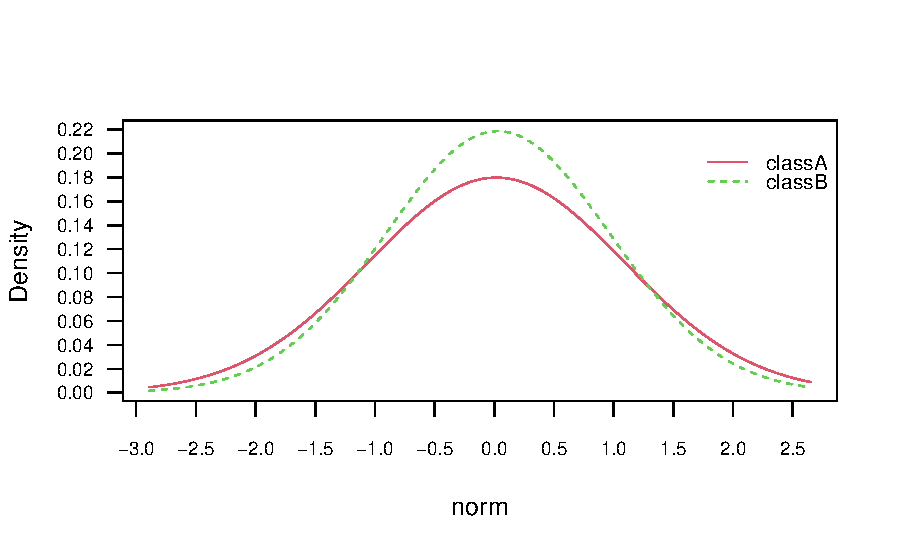
\includegraphics[width=\maxwidth]{figure/unnamed-chunk-4-1} 
\begin{kframe}\begin{alltt}
\hlcom{# Get names of assigned class conditional distributions}
\hlkwd{get_cond_dist}\hlstd{(nb)}
\end{alltt}
\begin{verbatim}
##          bern           cat       logical          norm         count 
##   "Bernoulli" "Categorical"   "Bernoulli"    "Gaussian"     "Poisson"
\end{verbatim}
\end{kframe}
\end{knitrout}


\subsection{Training with matrix/data.frame - vector interface}

The second example demonstrates model fitting and classification using the matrix/data.frame - vector interface. It involves simulating data with multiple predictors, fitting a Na\"ive Bayes model, summarizing the model, and performing classification on new data.

\begin{knitrout}
\definecolor{shadecolor}{rgb}{0.969, 0.969, 0.969}\color{fgcolor}\begin{kframe}
\begin{alltt}
\hlcom{# Section: Model fitting and classification using matrix/data.frame - vector interface}
\hlkwd{library}\hlstd{(naivebayes)}

\hlcom{# Simulate data}
\hlstd{n_vars} \hlkwb{<-} \hlnum{10}
\hlstd{n} \hlkwb{<-} \hlnum{1e6}
\hlstd{y} \hlkwb{<-} \hlkwd{sample}\hlstd{(}\hlkwc{x} \hlstd{=} \hlkwd{c}\hlstd{(}\hlstr{"a"}\hlstd{,} \hlstr{"b"}\hlstd{),} \hlkwc{size} \hlstd{= n,} \hlkwc{replace} \hlstd{=} \hlnum{TRUE}\hlstd{)}

\hlcom{# Discrete features}
\hlstd{X1} \hlkwb{<-} \hlkwd{matrix}\hlstd{(}\hlkwc{data} \hlstd{=} \hlkwd{sample}\hlstd{(letters[}\hlnum{5}\hlopt{:}\hlnum{9}\hlstd{], n} \hlopt{*} \hlstd{n_vars,} \hlnum{TRUE}\hlstd{),}
             \hlkwc{ncol} \hlstd{= n_vars)}
\hlstd{X1} \hlkwb{<-} \hlkwd{as.data.frame}\hlstd{(X1)}

\hlcom{# Fit a Naive Bayes model using matrix/data.frame - vector interface}
\hlstd{nb_cat} \hlkwb{<-} \hlkwd{naive_bayes}\hlstd{(}\hlkwc{x} \hlstd{= X1,} \hlkwc{y} \hlstd{= y)}

\hlcom{# Show summary of the model}
\hlkwd{summary}\hlstd{(nb_cat)}
\end{alltt}
\begin{verbatim}
## 
## ================================= Naive Bayes ================================== 
##  
## - Call: naive_bayes.default(x = X1, y = y) 
## - Laplace: 0 
## - Classes: 2 
## - Samples: 1000000 
## - Features: 10 
## - Conditional distributions: 
##     - Categorical: 10
## - Prior probabilities: 
##     - a: 0.5005
##     - b: 0.4995
## 
## --------------------------------------------------------------------------------
\end{verbatim}
\begin{alltt}
\hlcom{# Classification}
\hlkwd{system.time}\hlstd{(pred2} \hlkwb{<-} \hlkwd{predict}\hlstd{(nb_cat, X1))}
\end{alltt}
\begin{verbatim}
##    user  system elapsed 
##   0.301   0.021   0.323
\end{verbatim}
\begin{alltt}
\hlkwd{head}\hlstd{(pred2)}
\end{alltt}
\begin{verbatim}
## [1] a a b a b a
## Levels: a b
\end{verbatim}
\end{kframe}
\end{knitrout}


\subsection{Specialized Gaussian Naive Bayes}

This example focuses on showcasing the functionalities of the \textcolor{darkgreen}{{\btt{gaussian\_naive\_bayes()}}} function, which is specifically designed for handling continuous data with Gaussian distribution assumptions. It includes steps such as data preparation, model fitting, summary, and classification, providing insights into the practical application of this specialized function. Other specialized fitting functions have analogous interface.


\begin{knitrout}
\definecolor{shadecolor}{rgb}{0.969, 0.969, 0.969}\color{fgcolor}\begin{kframe}
\begin{alltt}
\hlcom{# Section: Model estimation through a specialized fitting function}
\hlkwd{library}\hlstd{(naivebayes)}

\hlcom{# Prepare data (matrix and vector inputs are strictly necessary)}
\hlkwd{data}\hlstd{(iris)}
\hlstd{M} \hlkwb{<-} \hlkwd{as.matrix}\hlstd{(iris[,} \hlnum{1}\hlopt{:}\hlnum{4}\hlstd{])}
\hlstd{y} \hlkwb{<-} \hlstd{iris}\hlopt{$}\hlstd{Species}

\hlcom{# Train the Gaussian Naive Bayes}
\hlstd{gnb} \hlkwb{<-} \hlkwd{gaussian_naive_bayes}\hlstd{(}\hlkwc{x} \hlstd{= M,} \hlkwc{y} \hlstd{= y)}
\hlkwd{summary}\hlstd{(gnb)}
\end{alltt}
\begin{verbatim}
## 
## ============================= Gaussian Naive Bayes ============================= 
##  
## - Call: gaussian_naive_bayes(x = M, y = y) 
## - Samples: 150 
## - Features: 4 
## - Prior probabilities: 
##     - setosa: 0.3333
##     - versicolor: 0.3333
##     - virginica: 0.3333
## 
## --------------------------------------------------------------------------------
\end{verbatim}
\begin{alltt}
\hlcom{# Parameter estimates}
\hlkwd{coef}\hlstd{(gnb)}
\end{alltt}
\begin{verbatim}
##              setosa:mu setosa:sd versicolor:mu versicolor:sd virginica:mu
## Sepal.Length     5.006 0.3524897         5.936     0.5161711        6.588
## Sepal.Width      3.428 0.3790644         2.770     0.3137983        2.974
## Petal.Length     1.462 0.1736640         4.260     0.4699110        5.552
## Petal.Width      0.246 0.1053856         1.326     0.1977527        2.026
##              virginica:sd
## Sepal.Length    0.6358796
## Sepal.Width     0.3224966
## Petal.Length    0.5518947
## Petal.Width     0.2746501
\end{verbatim}
\begin{alltt}
\hlkwd{coef}\hlstd{(gnb)[}\hlkwd{c}\hlstd{(}\hlnum{TRUE}\hlstd{,} \hlnum{FALSE}\hlstd{)]} \hlcom{# show only means}
\end{alltt}
\begin{verbatim}
##              setosa:mu versicolor:mu virginica:mu
## Sepal.Length     5.006         5.936        6.588
## Sepal.Width      3.428         2.770        2.974
## Petal.Length     1.462         4.260        5.552
## Petal.Width      0.246         1.326        2.026
\end{verbatim}
\begin{alltt}
\hlkwd{tables}\hlstd{(gnb,} \hlnum{1}\hlstd{)}
\end{alltt}
\begin{verbatim}
## -------------------------------------------------------------------------------- 
## :: Sepal.Length (Gaussian) 
## -------------------------------------------------------------------------------- 
##       setosa versicolor virginica
## mu 5.0060000  5.9360000 6.5880000
## sd 0.3524897  0.5161711 0.6358796
## 
## --------------------------------------------------------------------------------
\end{verbatim}
\begin{alltt}
\hlcom{# Visualization of fitted distributions}
\hlkwd{plot}\hlstd{(gnb,} \hlkwc{which} \hlstd{=} \hlnum{1}\hlstd{)}
\end{alltt}
\end{kframe}
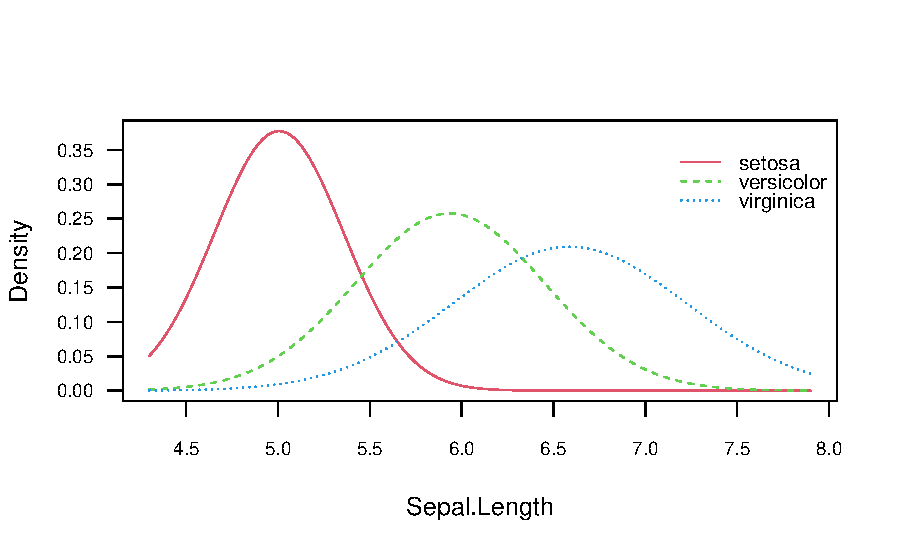
\includegraphics[width=\maxwidth]{figure/unnamed-chunk-6-1} 
\begin{kframe}\begin{alltt}
\hlcom{# Classification}
\hlkwd{head}\hlstd{(}\hlkwd{predict}\hlstd{(gnb,} \hlkwc{newdata} \hlstd{= M,} \hlkwc{type} \hlstd{=} \hlstr{"class"}\hlstd{))} \hlcom{# head(gnb %class% M)}
\end{alltt}
\begin{verbatim}
## [1] setosa setosa setosa setosa setosa setosa
## Levels: setosa versicolor virginica
\end{verbatim}
\begin{alltt}
\hlcom{# Posterior probabilities}
\hlkwd{head}\hlstd{(}\hlkwd{predict}\hlstd{(gnb,} \hlkwc{newdata} \hlstd{= M,} \hlkwc{type} \hlstd{=} \hlstr{"prob"}\hlstd{))} \hlcom{# head(gnb %prob% M)}
\end{alltt}
\begin{verbatim}
##      setosa   versicolor    virginica
## [1,]      1 2.981309e-18 2.152373e-25
## [2,]      1 3.169312e-17 6.938030e-25
## [3,]      1 2.367113e-18 7.240956e-26
## [4,]      1 3.069606e-17 8.690636e-25
## [5,]      1 1.017337e-18 8.885794e-26
## [6,]      1 2.717732e-14 4.344285e-21
\end{verbatim}
\begin{alltt}
\hlcom{# Equivalent calculation via naive_bayes}
\hlstd{gnb2} \hlkwb{<-} \hlkwd{naive_bayes}\hlstd{(M, y)}
\hlkwd{head}\hlstd{(}\hlkwd{predict}\hlstd{(gnb2,} \hlkwc{newdata} \hlstd{= M,} \hlkwc{type} \hlstd{=} \hlstr{"prob"}\hlstd{))}
\end{alltt}
\begin{verbatim}
##      setosa   versicolor    virginica
## [1,]      1 2.981309e-18 2.152373e-25
## [2,]      1 3.169312e-17 6.938030e-25
## [3,]      1 2.367113e-18 7.240956e-26
## [4,]      1 3.069606e-17 8.690636e-25
## [5,]      1 1.017337e-18 8.885794e-26
## [6,]      1 2.717732e-14 4.344285e-21
\end{verbatim}
\end{kframe}
\end{knitrout}


\break

\section{Appendix}

\subsection{Practical examples: parameter estimation}

This subsection provides a practical demonstration of parameter estimation in the Na\"ive Bayes model. It is aimed at students who are learning about the technical aspects of model fitting for the first time.

\subsubsection{Categorical distribution}

In this example, the well-known \textcolor{darkgreen}{{\btt{iris}}} dataset is modified by introducing a random categorical feature called "new" with 3 levels/categories. The parameters are then estimated using Maximum-Likelihood Estimation (MLE) and Bayesian estimation with pseudo-counts.

It's important to highlight that the example is intentionally designed to have one level with a very low probability of occurrence, which may not appear in the sample. Consequently, MLE may fail to provide a meaningful estimate for this level, resulting in a 0 probability estimate. This situation could lead to misleading results since it implies that the event is impossible, which might not be the case. Moreover, assigning a 0 probability to a category makes the calculation of posterior probabilities misleading, as it effectively renders the posterior probability 0 regardless of the probabilities assigned by other features.

In contrast, Bayesian estimation with the addition of pseudo counts offers a more reliable estimate, ensuring that even unlikely levels receive non-zero probabilities.

\begin{knitrout}
\definecolor{shadecolor}{rgb}{0.969, 0.969, 0.969}\color{fgcolor}\begin{kframe}
\begin{alltt}
\hlkwd{library}\hlstd{(naivebayes)}

\hlcom{# Prepare data: --------------------------------------------------------}
\hlkwd{data}\hlstd{(iris)}
\hlstd{iris2} \hlkwb{<-} \hlstd{iris}
\hlstd{N} \hlkwb{<-} \hlkwd{nrow}\hlstd{(iris2)}
\hlstd{n_new_factors} \hlkwb{<-} \hlnum{3}
\hlstd{factor_names} \hlkwb{<-} \hlkwd{paste0}\hlstd{(}\hlstr{"level"}\hlstd{,} \hlnum{1}\hlopt{:}\hlstd{n_new_factors)}

\hlcom{# Add a new categorical feature, where one level is very unlikely}
\hlkwd{set.seed}\hlstd{(}\hlnum{2}\hlstd{)}
\hlstd{iris2}\hlopt{$}\hlstd{new} \hlkwb{<-} \hlkwd{factor}\hlstd{(}\hlkwd{sample}\hlstd{(}\hlkwd{paste0}\hlstd{(}\hlstr{"level"}\hlstd{,} \hlnum{1}\hlopt{:}\hlstd{n_new_factors),}
                           \hlkwc{prob} \hlstd{=} \hlkwd{c}\hlstd{(}\hlnum{0.005}\hlstd{,} \hlnum{0.7}\hlstd{,} \hlnum{0.295}\hlstd{),}
                           \hlkwc{size} \hlstd{=} \hlnum{150}\hlstd{,}
                           \hlkwc{replace} \hlstd{=} \hlnum{TRUE}\hlstd{),} \hlkwc{levels} \hlstd{= factor_names)}

\hlcom{# Define class and feature levels: -------------------------------------}
\hlstd{Ck} \hlkwb{<-} \hlstr{"setosa"}
\hlstd{level1} \hlkwb{<-} \hlstr{"level1"}
\hlstd{level2} \hlkwb{<-} \hlstr{"level2"}
\hlstd{level3} \hlkwb{<-} \hlstr{"level3"}

\hlcom{# level1 did not show up in the sample but we know that it}
\hlcom{# has 0.5% probability to occur.}
\hlkwd{table}\hlstd{(iris2}\hlopt{$}\hlstd{new)}

\hlcom{# Parameter estimation: ------------------------------------------------}

\hlcom{# ML-estimates}
\hlstd{ck_sub_sample} \hlkwb{<-} \hlkwd{table}\hlstd{(iris2}\hlopt{$}\hlstd{new[iris}\hlopt{$}\hlstd{Species} \hlopt{==} \hlstd{Ck])}
\hlstd{ck_mle} \hlkwb{<-}  \hlstd{ck_sub_sample} \hlopt{/} \hlkwd{sum}\hlstd{(ck_sub_sample)}

\hlcom{# Bayesian estimation via symmetric Dirichlet prior with concentration parameter 0.5}
\hlcom{# (corresponds to the Jeffreys' uninformative prior)}

\hlstd{laplace} \hlkwb{<-} \hlnum{0.5}
\hlstd{N1} \hlkwb{<-} \hlkwd{sum}\hlstd{(iris2}\hlopt{$}\hlstd{Species} \hlopt{==} \hlstd{Ck} \hlopt{&} \hlstd{iris2}\hlopt{$}\hlstd{new} \hlopt{==} \hlstd{level1)} \hlopt{+} \hlstd{laplace}
\hlstd{N2} \hlkwb{<-} \hlkwd{sum}\hlstd{(iris2}\hlopt{$}\hlstd{Species} \hlopt{==} \hlstd{Ck} \hlopt{&} \hlstd{iris2}\hlopt{$}\hlstd{new} \hlopt{==} \hlstd{level2)} \hlopt{+} \hlstd{laplace}
\hlstd{N3} \hlkwb{<-} \hlkwd{sum}\hlstd{(iris2}\hlopt{$}\hlstd{Species} \hlopt{==} \hlstd{Ck} \hlopt{&} \hlstd{iris2}\hlopt{$}\hlstd{new} \hlopt{==} \hlstd{level3)} \hlopt{+} \hlstd{laplace}
\hlstd{N} \hlkwb{<-}  \hlkwd{sum}\hlstd{(iris2}\hlopt{$}\hlstd{Species} \hlopt{==} \hlstd{Ck)} \hlopt{+} \hlstd{laplace} \hlopt{*} \hlstd{n_new_factors}
\hlstd{ck_bayes} \hlkwb{<-} \hlkwd{c}\hlstd{(N1, N2, N3)} \hlopt{/} \hlstd{N}

\hlcom{# Compare estimates}
\hlkwd{rbind}\hlstd{(ck_mle, ck_bayes)}

\hlcom{# Unlike MLE, the Bayesian estimate for level1 assigns positive probability}
\hlcom{# but is slightly overestimated. Compared to MLE,}
\hlcom{# estimates for level2 and level3 have been slightly shrunken.}

\hlcom{# In general, the higher value of laplace, the more resulting}
\hlcom{# distribution tends to the uniform distribution.}
\hlcom{# When laplace would be set to infinity}
\hlcom{# then the estimates for level1, level2 and level3}
\hlcom{# would be 1/3, 1/3 and 1/3.}

\hlcom{# Comparison with estimates obtained with naive_bayes function:}
\hlstd{nb_mle} \hlkwb{<-} \hlkwd{naive_bayes}\hlstd{(Species} \hlopt{~} \hlstd{new,} \hlkwc{data} \hlstd{= iris2)}
\hlstd{nb_bayes} \hlkwb{<-} \hlkwd{naive_bayes}\hlstd{(Species} \hlopt{~} \hlstd{new,} \hlkwc{data} \hlstd{= iris2,} \hlkwc{laplace} \hlstd{= laplace)}

\hlcom{# MLE}
\hlkwd{rbind}\hlstd{(ck_mle,}
      \hlstr{"nb_mle"} \hlstd{=} \hlkwd{tables}\hlstd{(nb_mle,} \hlkwc{which} \hlstd{=} \hlstr{"new"}\hlstd{)[[}\hlnum{1}\hlstd{]][ ,Ck])}

\hlcom{# Bayes}
\hlkwd{rbind}\hlstd{(ck_bayes,}
      \hlstr{"nb_bayes"} \hlstd{=} \hlkwd{tables}\hlstd{(nb_bayes,} \hlkwc{which} \hlstd{=} \hlstr{"new"}\hlstd{)[[}\hlnum{1}\hlstd{]][ ,Ck])}


\hlcom{# Impact of 0 probabilities on posterior probabilities:}
\hlstd{new_data} \hlkwb{<-} \hlkwd{data.frame}\hlstd{(}\hlkwc{new} \hlstd{=} \hlkwd{c}\hlstd{(}\hlstr{"level1"}\hlstd{,} \hlstr{"level2"}\hlstd{,} \hlstr{"level3"}\hlstd{))}

\hlcom{# The posterior probabilities are NaNs, due to division by 0 when normalization}
\hlkwd{predict}\hlstd{(nb_mle, new_data,} \hlkwc{type} \hlstd{=} \hlstr{"prob"}\hlstd{,} \hlkwc{threshold} \hlstd{=} \hlnum{0}\hlstd{)}

\hlcom{# By default, this is remediated by replacing zero probabilities}
\hlcom{# with a small number given by threshold.}
\hlcom{# This leads to posterior probabilities being equal to prior probabilities}
\hlkwd{predict}\hlstd{(nb_mle, new_data,} \hlkwc{type} \hlstd{=} \hlstr{"prob"}\hlstd{)}
\end{alltt}
\end{kframe}
\end{knitrout}


\subsubsection{Gaussian distribution}

In this example, the famous \textcolor{darkgreen}{{\btt{iris}}} dataset is again used to demonstrate the Maximum-Likelihood estimation of the mean and variance in class conditional Gaussian distributions.

\begin{knitrout}
\definecolor{shadecolor}{rgb}{0.969, 0.969, 0.969}\color{fgcolor}\begin{kframe}
\begin{alltt}
\hlcom{# Prepare data: --------------------------------------------------------}
\hlkwd{data}\hlstd{(iris)}

\hlcom{# Define the feature and class of interest}
\hlstd{Xi} \hlkwb{<-} \hlstr{"Petal.Width"} \hlcom{# Selected feature}
\hlstd{Ck} \hlkwb{<-} \hlstr{"versicolor"}  \hlcom{# Selected class}

\hlcom{# Build class sub-sample for the selected feature}
\hlstd{Ck_Xi_subsample} \hlkwb{<-} \hlstd{iris[iris}\hlopt{$}\hlstd{Species} \hlopt{==} \hlstd{Ck, Xi]}

\hlcom{# Maximum-Likelihood Estimation (MLE)}
\hlstd{mle_norm} \hlkwb{<-} \hlkwd{cbind}\hlstd{(}\hlstr{"mean"} \hlstd{=} \hlkwd{mean}\hlstd{(Ck_Xi_subsample),}
                  \hlstr{"sd"} \hlstd{=} \hlkwd{sd}\hlstd{(Ck_Xi_subsample))}

\hlcom{# MLE estimates obtained using the naive_bayes function}
\hlstd{nb_mle} \hlkwb{<-} \hlkwd{naive_bayes}\hlstd{(}\hlkwc{x} \hlstd{= iris[Xi],} \hlkwc{y} \hlstd{= iris[[}\hlstr{"Species"}\hlstd{]])}
\hlkwd{rbind}\hlstd{(mle_norm,}
      \hlstr{"nb_mle"} \hlstd{=} \hlkwd{tables}\hlstd{(nb_mle,} \hlkwc{which} \hlstd{= Xi)[[Xi]][ ,Ck])}
\end{alltt}
\end{kframe}
\end{knitrout}


\subsubsection{Kernel Density Estimation}

In this example, kernel density estimation (KDE) is used to estimate class conditional densities for Sepal.Width variable from the \textcolor{darkgreen}{{\btt{iris}}} dataset.


\begin{knitrout}
\definecolor{shadecolor}{rgb}{0.969, 0.969, 0.969}\color{fgcolor}\begin{kframe}
\begin{alltt}
\hlcom{# Prepare data: --------------------------------------------------------}
\hlkwd{data}\hlstd{(iris)}

\hlcom{# Selected feature}
\hlstd{Xi} \hlkwb{<-} \hlstr{"Sepal.Width"}

\hlcom{# Classes}
\hlstd{C1} \hlkwb{<-} \hlstr{"setosa"}
\hlstd{C2} \hlkwb{<-} \hlstr{"virginica"}
\hlstd{C3} \hlkwb{<-} \hlstr{"versicolor"}

\hlcom{# Build class sub-samples for the selected feature}
\hlstd{C1_Xi_subsample} \hlkwb{<-} \hlstd{iris[iris}\hlopt{$}\hlstd{Species} \hlopt{==} \hlstd{C1, Xi]}
\hlstd{C2_Xi_subsample} \hlkwb{<-} \hlstd{iris[iris}\hlopt{$}\hlstd{Species} \hlopt{==} \hlstd{C2, Xi]}
\hlstd{C3_Xi_subsample} \hlkwb{<-} \hlstd{iris[iris}\hlopt{$}\hlstd{Species} \hlopt{==} \hlstd{C3, Xi]}

\hlcom{# Estimate class conditional densities for the selected feature}
\hlstd{dens1} \hlkwb{<-} \hlkwd{density}\hlstd{(C1_Xi_subsample)}
\hlstd{dens2} \hlkwb{<-} \hlkwd{density}\hlstd{(C2_Xi_subsample)}
\hlstd{dens3} \hlkwb{<-} \hlkwd{density}\hlstd{(C3_Xi_subsample)}

\hlcom{# Visualisation: -------------------------------------------------------}
\hlkwd{plot}\hlstd{(dens1,} \hlkwc{main} \hlstd{=} \hlstr{""}\hlstd{,} \hlkwc{col} \hlstd{=} \hlstr{"blue"}\hlstd{,} \hlkwc{xlim} \hlstd{=} \hlkwd{c}\hlstd{(}\hlnum{1.5}\hlstd{,} \hlnum{5}\hlstd{),} \hlkwc{ylim} \hlstd{=} \hlkwd{c}\hlstd{(}\hlnum{0}\hlstd{,} \hlnum{1.4}\hlstd{))}
\hlkwd{lines}\hlstd{(dens2,} \hlkwc{main} \hlstd{=} \hlstr{""}\hlstd{,} \hlkwc{col} \hlstd{=} \hlstr{"red"}\hlstd{)}
\hlkwd{lines}\hlstd{(dens3,} \hlkwc{main} \hlstd{=} \hlstr{""}\hlstd{,} \hlkwc{col} \hlstd{=} \hlstr{"black"}\hlstd{)}
\hlkwd{legend}\hlstd{(}\hlstr{"topleft"}\hlstd{,} \hlkwc{legend} \hlstd{=} \hlkwd{c}\hlstd{(C1, C2, C3),}
       \hlkwc{col} \hlstd{=} \hlkwd{c}\hlstd{(}\hlstr{"blue"}\hlstd{,} \hlstr{"red"}\hlstd{,} \hlstr{"black"}\hlstd{),}
       \hlkwc{lty} \hlstd{=} \hlnum{1}\hlstd{,} \hlkwc{bty} \hlstd{=} \hlstr{"n"}\hlstd{)}

\hlcom{# Compare to the naive_bayes: ------------------------------------------}
\hlstd{nb_kde} \hlkwb{<-} \hlkwd{naive_bayes}\hlstd{(}\hlkwc{x} \hlstd{= iris[Xi],} \hlkwc{y} \hlstd{= iris[[}\hlstr{"Species"}\hlstd{]],} \hlkwc{usekernel} \hlstd{=} \hlnum{TRUE}\hlstd{)}
\hlkwd{plot}\hlstd{(nb_kde,} \hlkwc{prob} \hlstd{=} \hlstr{"conditional"}\hlstd{)}

\hlstd{dens3}
\hlstd{nb_kde}\hlopt{$}\hlstd{tables[[Xi]][[C3]]}
\hlkwd{tables}\hlstd{(nb_kde, Xi)[[}\hlnum{1}\hlstd{]][[C3]]}


\hlcom{# Use custom bandwidth selector: ---------------------------------------}
\hlopt{?}\hlstd{bw.SJ}
\hlstd{nb_kde_SJ_bw} \hlkwb{<-} \hlkwd{naive_bayes}\hlstd{(}\hlkwc{x} \hlstd{= iris[Xi],} \hlkwc{y} \hlstd{= iris[[}\hlstr{"Species"}\hlstd{]],}
                      \hlkwc{usekernel} \hlstd{=} \hlnum{TRUE}\hlstd{,} \hlkwc{bw} \hlstd{=} \hlstr{"SJ"}\hlstd{)}
\hlkwd{plot}\hlstd{(nb_kde,} \hlkwc{prob} \hlstd{=} \hlstr{"conditional"}\hlstd{)}


\hlcom{# Visualize all available kernels: -------------------------------------}
\hlstd{kernels} \hlkwb{<-} \hlkwd{c}\hlstd{(}\hlstr{"gaussian"}\hlstd{,} \hlstr{"epanechnikov"}\hlstd{,} \hlstr{"rectangular"}\hlstd{,}\hlstr{"triangular"}\hlstd{,}
            \hlstr{"biweight"}\hlstd{,} \hlstr{"cosine"}\hlstd{,} \hlstr{"optcosine"}\hlstd{)}
\hlstd{iris3} \hlkwb{<-} \hlstd{iris}
\hlstd{iris3}\hlopt{$}\hlstd{one} \hlkwb{<-} \hlnum{1}

\hlkwd{sapply}\hlstd{(kernels,} \hlkwa{function} \hlstd{(}\hlkwc{ith_kernel}\hlstd{) \{}
    \hlstd{nb} \hlkwb{<-} \hlkwd{naive_bayes}\hlstd{(}\hlkwc{formula} \hlstd{= Species} \hlopt{~} \hlstd{one,} \hlkwc{data} \hlstd{= iris3,}
                      \hlkwc{usekernel} \hlstd{=} \hlnum{TRUE}\hlstd{,} \hlkwc{kernel} \hlstd{= ith_kernel)}
    \hlkwd{plot}\hlstd{(nb,} \hlkwc{arg.num} \hlstd{=} \hlkwd{list}\hlstd{(}\hlkwc{main} \hlstd{=} \hlkwd{paste0}\hlstd{(}\hlstr{"Kernel: "}\hlstd{, ith_kernel),}
                            \hlkwc{col} \hlstd{=} \hlstr{"black"}\hlstd{),} \hlkwc{legend} \hlstd{=} \hlnum{FALSE}\hlstd{)}
    \hlkwd{invisible}\hlstd{()}
\hlstd{\})}
\end{alltt}
\end{kframe}
\end{knitrout}

\subsubsection{Poisson distribution}

This example illustrates the parameter estimation for class conditional Poisson features based on simulated data.

\begin{knitrout}
\definecolor{shadecolor}{rgb}{0.969, 0.969, 0.969}\color{fgcolor}\begin{kframe}
\begin{alltt}
\hlcom{# Simulate data: -------------------------------------------------------}
\hlstd{cols} \hlkwb{<-} \hlnum{2}
\hlstd{rows} \hlkwb{<-} \hlnum{10}
\hlkwd{set.seed}\hlstd{(}\hlnum{11}\hlstd{)}
\hlstd{M} \hlkwb{<-} \hlkwd{matrix}\hlstd{(}\hlkwd{rpois}\hlstd{(rows} \hlopt{*} \hlstd{cols,} \hlkwc{lambda} \hlstd{=} \hlkwd{c}\hlstd{(}\hlnum{0.1}\hlstd{,}\hlnum{1}\hlstd{)),} \hlkwc{nrow} \hlstd{= rows,}
            \hlkwc{ncol} \hlstd{= cols,} \hlkwc{dimnames} \hlstd{=} \hlkwd{list}\hlstd{(}\hlkwa{NULL}\hlstd{,} \hlkwd{paste0}\hlstd{(}\hlstr{"Var"}\hlstd{,} \hlkwd{seq_len}\hlstd{(cols))))}
\hlstd{y} \hlkwb{<-} \hlkwd{factor}\hlstd{(}\hlkwd{sample}\hlstd{(}\hlkwd{paste0}\hlstd{(}\hlstr{"class"}\hlstd{, LETTERS[}\hlnum{1}\hlopt{:}\hlnum{2}\hlstd{]), rows,} \hlnum{TRUE}\hlstd{))}
\hlstd{Xi} \hlkwb{<-} \hlstd{M[ ,}\hlstr{"Var1"}\hlstd{,} \hlkwc{drop} \hlstd{=} \hlnum{FALSE}\hlstd{]}

\hlcom{# MLE: -----------------------------------------------------------------}
\hlcom{# Estimate lambdas for each class}
\hlkwd{tapply}\hlstd{(Xi, y, mean)}

\hlcom{# Compare with naive_bayes}
\hlstd{pnb} \hlkwb{<-} \hlkwd{naive_bayes}\hlstd{(}\hlkwc{x} \hlstd{= Xi,} \hlkwc{y} \hlstd{= y,} \hlkwc{usepoisson} \hlstd{=} \hlnum{TRUE}\hlstd{)}
\hlkwd{tables}\hlstd{(pnb,} \hlnum{1}\hlstd{)}

\hlcom{# Adding pseudo-counts via laplace parameter: --------------------------}
\hlstd{laplace} \hlkwb{<-} \hlnum{1}
\hlstd{Xi_pseudo} \hlkwb{<-} \hlstd{Xi}
\hlstd{Xi_pseudo[y} \hlopt{==} \hlstr{"classB"}\hlstd{,][}\hlnum{1}\hlstd{]} \hlkwb{<-} \hlstd{Xi_pseudo[y} \hlopt{==} \hlstr{"classB"}\hlstd{,][}\hlnum{1}\hlstd{]} \hlopt{+} \hlstd{laplace}
\hlstd{Xi_pseudo[y} \hlopt{==} \hlstr{"classA"}\hlstd{,][}\hlnum{1}\hlstd{]} \hlkwb{<-} \hlstd{Xi_pseudo[y} \hlopt{==} \hlstr{"classA"}\hlstd{,][}\hlnum{1}\hlstd{]} \hlopt{+} \hlstd{laplace}

\hlcom{# Estimates}
\hlkwd{tapply}\hlstd{(Xi_pseudo, y, mean)}

\hlcom{# Compare with naive_bayes}
\hlstd{pnb} \hlkwb{<-} \hlkwd{naive_bayes}\hlstd{(}\hlkwc{x} \hlstd{= Xi,} \hlkwc{y} \hlstd{= y,} \hlkwc{usepoisson} \hlstd{=} \hlnum{TRUE}\hlstd{,} \hlkwc{laplace} \hlstd{= laplace)}
\hlkwd{tables}\hlstd{(pnb,} \hlnum{1}\hlstd{)}
\end{alltt}
\end{kframe}
\end{knitrout}


\subsubsection{Multinomial distribution}

This example is based on simulated data generated for an artificial scenario. It simulates word counts for a collection of documents, distinguishing between spam and non-spam categories. The data generation process is artificial and does not represent real-world documents. It serves as a simplified illustration of estimating multinomial probabilities for each class.

\begin{knitrout}
\definecolor{shadecolor}{rgb}{0.969, 0.969, 0.969}\color{fgcolor}\begin{kframe}
\begin{alltt}
\hlcom{# Prepare data for an artificial example: --------------------------------------}
\hlkwd{set.seed}\hlstd{(}\hlnum{1}\hlstd{)}
\hlstd{cols} \hlkwb{<-} \hlnum{3}       \hlcom{# words}
\hlstd{rows} \hlkwb{<-} \hlnum{100}     \hlcom{# all documents}
\hlstd{rows_spam} \hlkwb{<-} \hlnum{10} \hlcom{# spam documents}

\hlcom{# Probability of no-spam for each word}
\hlstd{prob_non_spam} \hlkwb{<-} \hlkwd{prop.table}\hlstd{(}\hlkwd{runif}\hlstd{(cols))} \hlcom{# C_1}

\hlcom{# Probability of spam for each word}
\hlstd{prob_spam} \hlkwb{<-} \hlkwd{prop.table}\hlstd{(}\hlkwd{runif}\hlstd{(cols))} \hlcom{# C_2}

\hlcom{# Simulate counts of words according to the multinomial distributions}
\hlstd{M1} \hlkwb{<-} \hlkwd{t}\hlstd{(}\hlkwd{rmultinom}\hlstd{(rows} \hlopt{-} \hlstd{rows_spam,} \hlkwc{size} \hlstd{= cols,} \hlkwc{prob} \hlstd{= prob_non_spam))}
\hlstd{M2} \hlkwb{<-} \hlkwd{t}\hlstd{(}\hlkwd{rmultinom}\hlstd{(rows_spam,}        \hlkwc{size} \hlstd{= cols,} \hlkwc{prob} \hlstd{= prob_spam))}
\hlstd{M} \hlkwb{<-} \hlkwd{rbind}\hlstd{(M1, M2)}
\hlkwd{colnames}\hlstd{(M)} \hlkwb{<-} \hlkwd{paste0}\hlstd{(}\hlstr{"word"}\hlstd{,} \hlnum{1}\hlopt{:}\hlstd{cols) ;} \hlkwd{rownames}\hlstd{(M)} \hlkwb{<-} \hlkwd{paste0}\hlstd{(}\hlstr{"doc"}\hlstd{,} \hlnum{1}\hlopt{:}\hlstd{rows)}
\hlkwd{head}\hlstd{(M)}

\hlcom{# Simulate response with spam/no-spam}
\hlstd{y} \hlkwb{<-} \hlkwd{c}\hlstd{(}\hlkwd{rep}\hlstd{(}\hlstr{"non-spam"}\hlstd{, rows} \hlopt{-} \hlstd{rows_spam),} \hlkwd{rep}\hlstd{(}\hlstr{"spam"}\hlstd{, rows_spam))}

\hlcom{# Additive smoothing}
\hlstd{laplace} \hlkwb{<-} \hlnum{0.5}

\hlcom{# Estimate the multinomial probabilities p_\{ik\} (i is word, k is class)}
\hlcom{# p1 = (p_11, p_21, p_31) (non-spam)}
\hlcom{# p2 = (p_12, p_22, p_32) (spam)}

\hlstd{N_1} \hlkwb{<-} \hlkwd{sum}\hlstd{(M1)}
\hlstd{N_i1} \hlkwb{<-} \hlkwd{colSums}\hlstd{(M1)}
\hlstd{p1} \hlkwb{<-} \hlstd{(N_i1} \hlopt{+} \hlstd{laplace)} \hlopt{/} \hlstd{(N_1} \hlopt{+} \hlstd{cols} \hlopt{*} \hlstd{laplace)}

\hlstd{N_2} \hlkwb{<-} \hlkwd{sum}\hlstd{(M2)}
\hlstd{N_i2} \hlkwb{<-} \hlkwd{colSums}\hlstd{(M2)}
\hlstd{p2} \hlkwb{<-} \hlstd{(N_i2} \hlopt{+} \hlstd{laplace)} \hlopt{/} \hlstd{(N_2} \hlopt{+} \hlstd{cols} \hlopt{*} \hlstd{laplace)}

\hlcom{# Combine estimated Multinomial probabilities for each class}
\hlkwd{cbind}\hlstd{(}\hlstr{"non-spam"} \hlstd{= p1,} \hlstr{"spam"} \hlstd{= p2)}

\hlcom{# Compare to the multinomial_naive_bayes}
\hlstd{mnb} \hlkwb{<-} \hlkwd{multinomial_naive_bayes}\hlstd{(}\hlkwc{x} \hlstd{= M,} \hlkwc{y} \hlstd{= y,} \hlkwc{laplace} \hlstd{= laplace)}
\hlkwd{coef}\hlstd{(mnb)}
\hlcom{# colSums(coef(mnb))}
\end{alltt}
\end{kframe}
\end{knitrout}

\end{document}
